\documentclass{article}
\usepackage{fullpage,hyperref,url,setspace,graphicx,authblk,natbib}
\usepackage{subcaption}
\usepackage{lineno}
% \bibliography{references,R}
% \bibliographystyle{genetics}

\hypersetup{colorlinks=true,
linkcolor=blue,          % color of internal links (change box color with linkbordercolor)
citecolor=blue,        % color of links to bibliography
filecolor=blue,      % color of file links
urlcolor=blue           % color of external links
}
\doublespacing

\author[1]{Kevin R. Thornton}
\affil[1]{Department of Ecology and Evolutionary Biology, University of California Irvine}
\title{Improving forward-time simulation performance using succinct tree sequences.}

\begin{document}
\maketitle
\linenumbers

\section*{Abstract}
\section*{Introduction}

\newpage
\begin{figure}[!h]
    \centering
    \begin{subfigure}[b]{0.45\textwidth}
        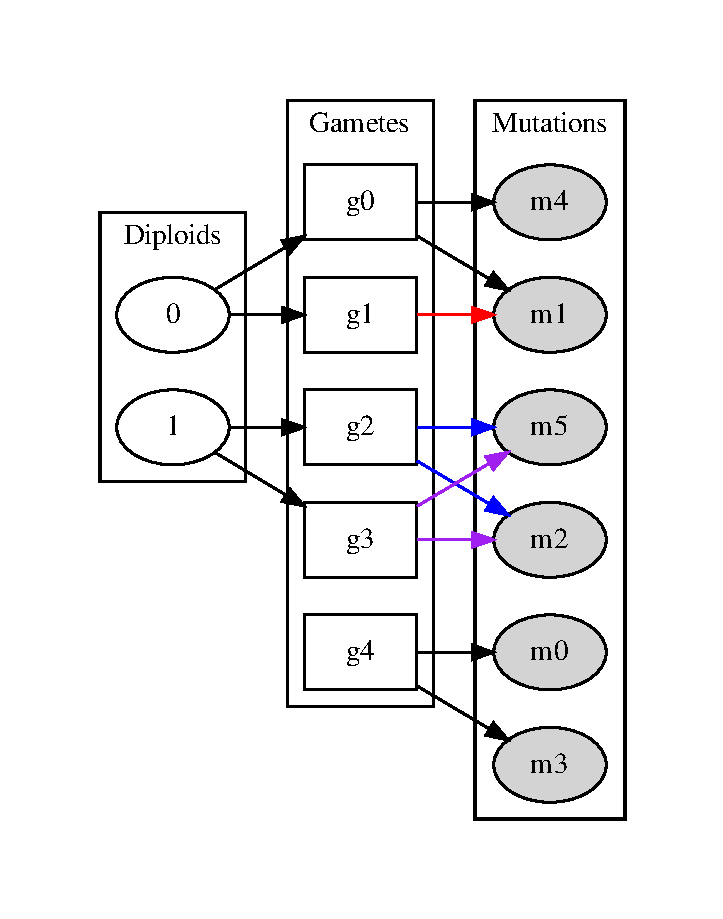
\includegraphics[scale=0.5]{figs/datastructures}
        \caption{\label{sfig:datastructures}Data structures used in \texttt{fwdpp}}
    \end{subfigure}
    \begin{subfigure}[b]{0.45\textwidth}
        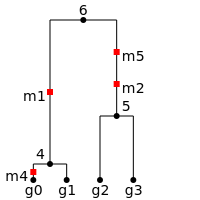
\includegraphics[scale=3]{figs/tree}
        \caption{\label{sfig:tree}Representing the data structures as a tree}
    \end{subfigure}
    \caption{\label{fig:datatree}How gametes and mutations in a population map to nodes on a tree.}
\end{figure}
\newpage
\bibliography{references}
\bibliographystyle{genetics}

\end{document}
